\documentclass{article}

\usepackage{graphicx} % Required for the inclusion of images
\usepackage{natbib} % Required to change bibliography style to APA
\usepackage{amsmath} % Required for some math elements 
\usepackage{url}
\usepackage{hyperref}
\usepackage{listings}
\usepackage{textcomp}
\usepackage[titletoc,title]{appendix}
\setlength\parindent{0pt} % Removes all indentation from paragraphs

\usepackage{geometry}
 \geometry{
 total={210mm,297mm},
 left=20mm,
 right=20mm,
 top=40mm,
 bottom=20mm,
 }

\title{RNA-Seq Analysis Report \\ {{project_id}}}
\author{Center For Cancer Computational Biology \\ Dana Farber Cancer Institute}

\begin{document}

\maketitle

\section{Introduction}
This report summarizes the analyses used in analyzing your data. For further questions regarding details of the analysis, please contact the CCCB.

\section{Experimental setup}

The following samples and their corresponding annotations were used in this analysis:

\begin{center}
    \begin{tabular}{c|c}
     Sample ID & Group \\ \hline
     
	{{id}} & {{group}}{{ "\\\\" }}
     
    \end{tabular}
\end{center}




The following pairwise group comparisons were performed:

\begin{center}
    \begin{tabular}{c|c}
     Base/Control & Experimental \\ \hline
     
	{{control_group}} & {{exp_group}}{{ "\\\\" }}
     
    \end{tabular}
\end{center}

If the contrast appears reversed in the table above, it does not affect the differential expression testing performed.  If this is the case the directions of differential expression become reversed but the significance of differential expression remains the same.



\section{Reference genome}
Your data was aligned against the {{ref_genome_name}} genome, available at \url {{'{'}} {{ ref_genome_url }} {{'}'}}



\section{Alignment}
Alignments were performed with STAR aligner  (version 2.3.1z4) \cite{star} which is specifically designed for RNA-Seq experiments, which may include multiple splice forms and fusion transcripts.  Not all aligners produce the same results, as sequencing mistake, low--complexity sequences, variants, and other factors are treated differently and may affect the quality of the resulting alignment to the reference genome.\\

The output from the alignment is in a compressed, binary format-- a BAM file.  Although not often necessary, text representations of the BAM file (SAM format) may be generated with software such as samtools \cite{samtools}.\\

Following the alignment, the BAM files are passed through several processing steps.  For our standard processes, we deliver three levels of BAM file:
\begin{itemize}
\item *.sort.bam \\
These BAM files are sorted by genomic coordinates, which is necessary for tools such as IGV (see Section \ref{sec:igv})
\item *.sort.primary.bam \\
To obtain these BAM files we filter the sorted BAM files to retain only ``primary'' alignments.  When sequencing reads are aligned to the reference genome, it is possible that they may align well to multiple locations due to homology, paralogous genes, low-complexity regions, sequencing errors, or any number of other factors.  The aligner scores the quality of the alignment and marks some reads as secondary.  Thus, the primary-filtered files retain only the most high-quality reads for downstream analysis.  We recommend using these BAM files for further downstream analysis.  
\item *.sort.primary.dedup.bam \\
These are BAM files which remove reads that are marked as duplicates.  Here, duplicates are defined as reads that align to the same exact genomic coordinates and have the same sequence.  In whole-genome DNA sequencing, the random fragmentation results in a very low probability of two identical pieces of DNA; reads that are exact copies are most likely artifacts of PCR amplification and should be discarded.  While PCR-based duplication is still a problem for low-quantity RNA-Seq experiments there is increasing evidence that the removal of duplicate reads unnecessarily discards good data, perhaps affecting the eventual testing for differential expression.  Since only a small portion of the genome is sampled in a RNA-Seq experiment, it is more likely that the fragmentation of distinct transcripts can result in identical RNA fragments.  Illumina has reported on internal studies which used unique sequence barcodes to distinguish PCR-based duplicates from duplicate reads originating from distinct transcripts.  Their data suggest that it is good practice to retain the duplicate reads.  However, it is important to appreciate that there is still some debate surrounding this matter.  
\end{itemize}

In our convention, the asterisk (*) is the sample identifier and there are three BAM files for each sample.
Brief alignment metrics are shown below in Figures \ref{fig:relative_composition} and \ref{fig:total_counts}:

\begin{figure}[ht!]
  \centering
    \includegraphics[width=0.75\textwidth]{mapping_composition}
    \caption{The relative composition of reads from alignment.}
    \label{fig:relative_composition}
\end{figure}

\begin{figure}[ht!]
  \centering
    \includegraphics[width=0.75\textwidth]{total_reads}
    \caption{The total reads from the experiment.}
     \label{fig:total_counts}
\end{figure}

\begin{figure}[ht!]
  \centering
    \includegraphics[width=0.75\textwidth]{bamfile_reads}
    \caption{The total reads at each filter level.}
     \label{fig:bam_level_counts}
\end{figure}



\section{RNA-Seq QC}

RNA-Seq quality metrics are produced by the Broad Institute's RNA-SeQC tool \cite{rnaseqc} (\url{http://www.broadinstitute.org/cancer/cga/rna-seqc}).  Please see their documentation for interpretation of any figures and metrics.

\section{Read quantification}

For this analysis, reads and differential expression analysis are treated at the gene level, as opposed to inference about specific transcript abundance.  Even at the simpler level of counting reads at the gene level, there are subtle issues in just how you perform this.  For this task we use featureCounts software \cite{featureCounts} which produces integer counts for all genes in the supplied genome annotation file (GTF format).  \\

The resulting counts are arranged into an expression matrix such as,
\begin{center}
\begin{tabular}{c || c | c | c | r }
  Gene & SampleA & SampleB & SampleC & \ldots \\
  \hline			
  X & 1 & 2 & 3 & \ldots \\
  Y & 4 & 5 & 6 & \ldots\\
  Z & 7 & 8 & 9 & \ldots\\
  \hline  
\end{tabular}
\end{center}

Files containing the information are termed the ``raw'' counts and are available at all three filter levels described for the BAM files.  These are tab-delimited files and may be opened with a spreadsheet program such as Excel.


\section{Read normalization}
\label{sec:normalization}

As seen in Figure \ref{fig:total_counts}, each sample has a different number of total reads to begin with.  Thus, we cannot simply compare the raw counts between samples to determine differential expression-- even genes that have similar expression would appear to be differentially expressed if the input library sizes were significantly different.\\

There are several popular methods for normalizing the count matrix to account for technical differences between samples.  The method used in this analysis is part of the DESeq \cite{deseq} package, one of R's Bioconductor suite of software tools.  Further information and implementation details can be found in the DESeq publication.  The DESeq normalization scheme looks for systematically different expression levels across samples and uses a robust median-based scaling.  A significant assumption (but often true in practice) is that most genes are \emph{not} differentially expressed.  Therefore, samples where many genes have higher (or lower) relative expression would indicate that an appropriate scaling should be performed.   \\

Normalized count files are formatted in the same manner as the raw count files and are available at all three levels of BAM file.  When comparing against the differential expression files (explained below), it is often helpful to look at the normalized count levels contained in these files.\\

We note that normalization measures such as RPKM/FPKM were quite popular in the past, but have since largely been replaced by integer-count based methods such as those in DESeq (and similar packages such as edgeR).




\section{Differential expression testing}

The concept behind RNA-Seq experiments is that we may use the relative abundance of sequencing reads to infer the relative quantities of RNA and hence determine differential expression across different biological states.  In general, the number of sequencing reads from a particular region of the genome is affected by a number of biases introduced in the protocols (e.g. PCR-based biases during library construction) and it is not appropriate to compare multiple genes \emph{within the same sample}.  For instance, genes with very different GC content may be amplified at different rates and any observed count differences are not due to the relative RNA amounts.  However, comparison of the same gene across multiple samples is reasonable since biases related to the sequence itself are largely removed.  Thus, the aim of the differential expression analysis is to compare expression of the same locus across multiple experiments or conditions.\\

For differential expression testing, we use DESeq software, as described in Section~\ref{sec:normalization}.  In short, this assumes that read abundances for a particular gene in a particular sample follow a \emph{negative-binomial distribution}.  The goal of the analysis is to infer model parameters such as the mean and variance based on the observed data.  In particular, DESeq uses a number of techniques to obtain estimates of these parameters despite the low number of samples available in most sequencing experiments (sometimes without any replicates, although such an experimental design is not ideal for strong evidence).  Finally, using these parameters, a significance (p-value) for differential expression is calculated. For further details, please consult the publication.\\  

The output files are named according to the contrast performed.  For example, \verb|X_vs_Y.sort.primary.deseq| compares group X versus group Y, treating Y as the ``base'' or ``control'' condition.  The actual order of comparison does not matter with regards to determining differential expression; it is, however, important to note the direction of differential regulation.  If the contrast is switched from your preference, then upregulation becomes downregulation and vice versa.  For example, given a file named \verb|X_vs_Y.sort.primary.deseq|, if gene YFG (Your Favorite Gene) has a fold-change of 5.3, this indicates that the expression of YFG is upregulated in condition X with respect to condition Y.  If, however, you wished to treat X as the control condition, then YFG would be downregulated at a fold-change of $1/5.3 = 0.19$.   \\

The values in the output files are comma-separated, and may be viewed by a spreadsheet program such as Excel.  The columns are as follows:
\begin{center}
\begin{tabular}{r|l}
id & The gene symbol \\
baseMean & A composite measure of the mean in both conditions  \\
\textlangle{}control id\textrangle{} & A measure of the mean in the control condition \\
\textlangle{}exp id\textrangle{} & A measure of the mean in the experimental condition \\
foldChange & The fold change (ratio)\\
log2FoldChange & The logarithm of the fold change \\
pval & The raw p-value from the differential expression test \\
padj & The multiple-test corrected p-value (see below)
\end{tabular}
\end{center}

Most often, investigators are interested in the most differentially expressed genes.  To view these, the simplest strategy is to sort the output files by the \verb|padj| column, which gives the multiple-test corrected p-value.  In short, the multiple-test correction attempts to limit the number of false discoveries; many methods are available, but DESeq uses the Benjamini-Hochberg correction; there are sources available online with further information on the multiple testing problem.  It is common to filter to retain only genes with \verb|padj| values less than 0.05, but this threshold is arbitrary and larger or smaller values may be used.\\

In general, you will note that genes with low abundance but high fold-change (e.g. counts of 1 and 10 in the two conditions) are not assigned very confident p-values; the typical variance in the read counts of a sequencing experiment may be larger than those values and the p-value reflects this fact.  In such a case it is difficult to determine if the change is due to actual differential expression or just the ``random error'' (sampling biases, inherent biological variability, etc.)  As the absolute magnitude of the counts become larger (e.g. counts of 500 and 1000), then the p-values will decrease accordingly, indicating more confidence in the determination of differential expression.  \\

For this experiment, we have the following number of genes (at the {{bam_filter_level}} level) marked as differentially expressed at the $\textrm{FDR} < 0.05$ threshold.:

\begin{center}
    \begin{tabular}{|c|c|c|c|}
    \hline
    \multicolumn{2}{|c|}{Contrast} &
    \multicolumn{2}{c|}{Number of Genes}\\ \hline
     Base/Control & Experimental & Upregulated & Downregulated\\ \hline
     
	{{control_group}} & {{exp_group}} & {{upregulated_count}} & {{downregulated_count}}{{ '\\\\' }}
     
     \hline
    \end{tabular}
\end{center}



\section{Viewing your alignment data}
\label{sec:igv}
For viewing the BAM files, we recommend downloading and installing the Integrated Genomics Viewer (IGV), released by the Broad Institute.  This software runs on platforms with a Java installation (Windows, Mac, Linux/Unix) and can help to view more informationa about your experiment, including detection of problems. \\

In Figure \ref{fig:igv_dups}, we have focused on a $~1800$bp region in an exon of the MALAT1 gene where one can see very non-uniform read distribution across this particular exon.  One location in particular has many sequencing reads stacked on top of one another, with very minimal random tiling/overlap.  In addition, the red color indicates that all the reads originated from a single strand.  A more typical alignment shown in Figure \ref{fig:igv_typical} shows a mix of plus and minus-strand reads and random tiling/overlap.

\begin{figure}[ht!]
  \centering
    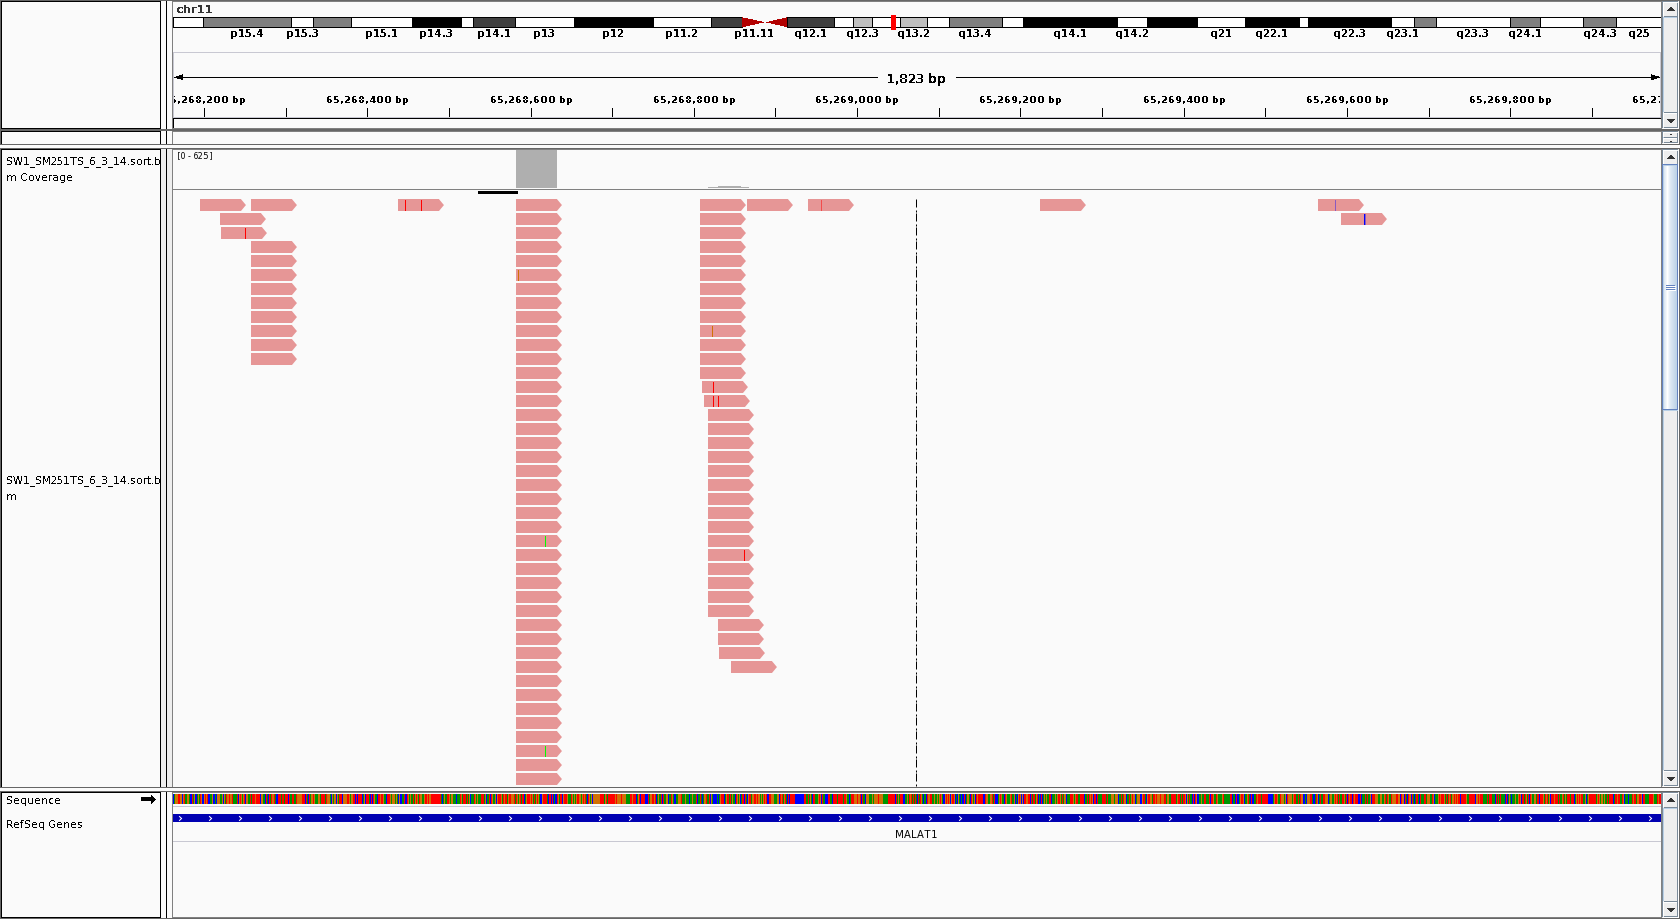
\includegraphics[width=0.75\textwidth]{igv_duplicates}
    \caption{IGV screenshot.  Many duplicate reads are visible.}
     \label{fig:igv_dups}
\end{figure}

\begin{figure}[ht!]
  \centering
    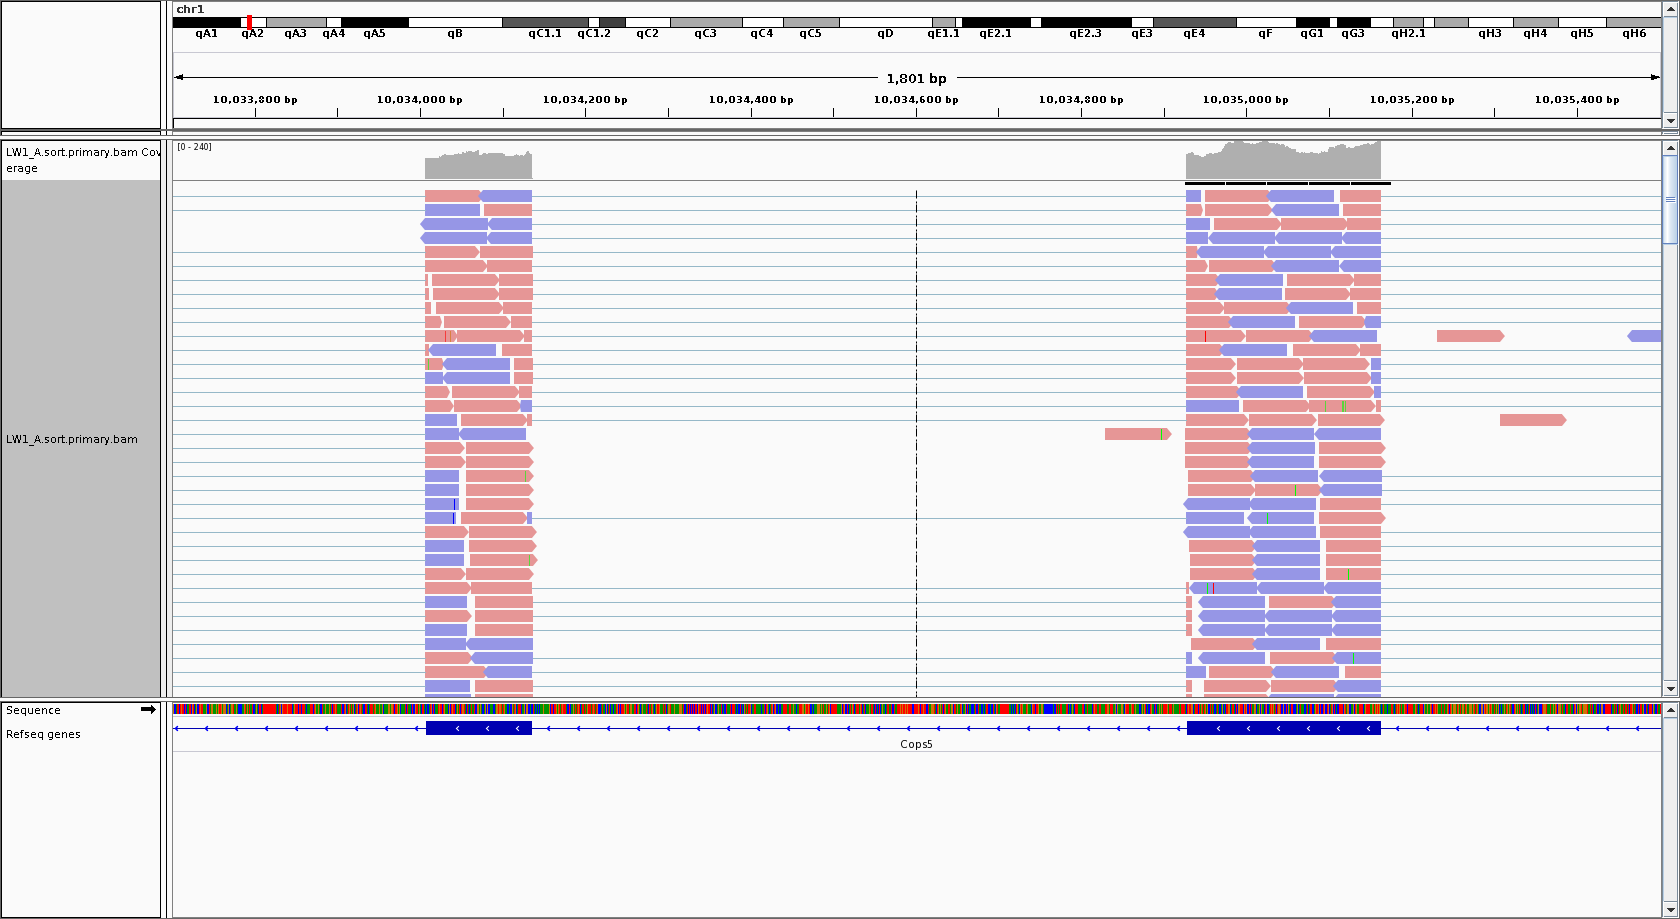
\includegraphics[width=0.75\textwidth]{igv_typical}
    \caption{IGV screenshot.  A more ``typical'' picture of read alignments.}
     \label{fig:igv_typical}
\end{figure}

\bibliographystyle{plain}

\bibliography{references}


\newpage
\appendix

\begin{appendices}



\section{Read coverage}

Depending on the desired outcomes of the sequencing experiment, different levels of sequencing coverage may be necessary to adequately answer the question.  Additionally, extremely variable coverage may indicate problems such as low RNA quantities and overamplification.  For example sample, we plot the coverage of each chromosome below.  Large spikes in the coverage profile could indicate high levels of duplicate reads and a problem with the experiment.


	\begin{figure}[ht!]
	  \centering
	    \includegraphics[width=0.85\textwidth]{{'{{{'}}{{cvg_plot}}{{'}}}'}}
	    \caption{Read coverage for sample {{sample_id}}}
	\end{figure}


\end{appendices}

\end{document}

